\documentclass{beamer}

\usepackage[utf8]{inputenc}
\usepackage{pgfpages}
\usepackage{mathtools}
\usepackage{array}
\usepackage{drs}
\input{qobitree}
\usepackage{listings}


\setbeamertemplate{navigation symbols}{}
\setbeamertemplate{footline}
  {\hfill {\normalsize \insertframenumber{}/\inserttotalframenumber{}}}
\hypersetup{pdfstartview={Fit}}

\AtBeginSection[]
{
\begin{frame}{Outline}
  \tableofcontents[currentsection]
\end{frame}
}

\newcommand{\hsbind}{\mathbin{\gg\!=}}
\newcommand{\apl}{\mathbin{\ll\!\!\cdot}}
\newcommand{\apr}{\mathbin{\cdot\!\!\gg}}
\newcommand{\aplr}{\mathbin{\ll\!\!\cdot\!\!\gg}}
\newcommand{\cons}{\mathbin{::}}
\newcommand{\cat}{\mathbin{+\mkern-10mu+}}

\newcommand{\abs}[1]{\textsc{#1}}
\newcommand{\obj}[1]{\textbf{#1}}
\newcommand{\sem}[1]{\llbracket #1 \rrbracket}
\newcommand{\lex}[2]{\sem{\abs{#1}} &:= #2}

\newcommand{\semdom}[1]{\textbf{#1}}

\newcommand{\dand}{\mathbin{\overline{\land}}}
\newcommand{\dnot}{\mathop{\overline{\lnot}}}
\newcommand{\dor}{\mathop{\overline{\lor}}}
\newcommand{\dimpl}{\mathbin{\overline{\to}}}
\newcommand{\dexists}{\mathop{\overline{\exists}}}
\newcommand{\dforall}{\mathop{\overline{\forall}}}

\newcommand{\limp}{\mathbin{{-}\mkern-3.5mu{\circ}}}

\newcommand{\llbparenthesis}{\vcenter{\hbox{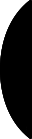
\includegraphics{symbols/llbparenthesis.png}}}}
\newcommand{\rrbparenthesis}{\vcenter{\hbox{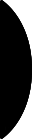
\includegraphics{symbols/rrbparenthesis.png}}}}
\newcommand{\lban}{\llparenthesis \,}
\newcommand{\rban}{\, \rrparenthesis}
\newcommand{\lbban}{\llbparenthesis \,}
\newcommand{\rbban}{\, \rrbparenthesis}
\newcommand{\banana}[1]{\lban #1 \rban}
\newcommand{\bbanana}[1]{\lbban #1 \rbban}
\newcommand{\cherry}{\rotatebox[origin=c]{270}{$\limp$}}

\newcommand{\lam}[2]{\lambda #1.\, #2}
\newcommand{\ap}[2]{#1\,#2}
\newcommand{\app}[3]{\ap{\ap{#1}{#2}}{#3}}
\newcommand{\appp}[4]{\ap{\ap{\ap{#1}{#2}}{#3}}{#4}}
\newcommand{\op}[1]{\mathtt{#1}}
\newcommand{\onto}[1]{#1 \mathalpha{:\,}}
\newcommand{\typedop}[3]{\op{#1} : #2 \rightarrowtail #3}
\newcommand{\typedopg}[3]{#1 : #2 \rightarrowtail #3}
\newcommand{\row}[2]{\{ #1 \mathrel{|} #2 \}}

\newcommand{\CC}{\mathcal{C}}
\newcommand{\FF}{\mathcal{F}}
\newcommand{\XX}{\mathcal{X}}
\newcommand{\EE}{\mathcal{E}}
\newcommand{\TT}{\mathcal{T}}
\newcommand{\PP}{\mathcal{P}}

\newcommand{\FV}{\operatorname{FV}}

\newcommand{\subst}[3]{#1[#2 \coloneqq #3]}

\newcommand{\syntclos}[1]{\mathbin{[#1]}}





\newcommand{\cibanana}{\banana{(\onto{\op{op}_i} M_i)_{i \in I},\ \onto{\eta} M_\eta}}
\newcommand{\cdbanana}{\banana{\onto{\op{op}_1} M_1,\ \dots,\ \onto{\op{op}_n} M_n,\ \onto{\eta} M_\eta}}

\newcommand{\cibbanana}{\bbanana{(\onto{\op{op}_i} M_i)_{i \in I},\ \onto{\eta} M_\eta}}

\newcommand{\TODO}[1]{\textcolor{red}{\textbf{TODO}: #1}}

\newcommand{\relR}{\mathbin{R}}

\newcommand{\swap}{\mathbin{\textbf{swap}}}

\newcommand{\tto}{\twoheadrightarrow}

\mathchardef\mhyphen="2D

\newcommand{\pair}[2]{\left<#1, #2\right>}
\newcommand{\inl}{\operatorname{inl}}
\newcommand{\inr}{\operatorname{inr}}
\newcommand{\case}[5]{\text{\textbf{case} $#1$ \textbf{of} $\{ \ap{\inl}{#2} \to #3;\ \ap{\inr}{#4} \to #5 \}$}}
\newcommand{\absurd}[1]{\text{\textbf{case} $#1$ \textbf{of} \{\,\}}}

\newcommand{\true}{\textbf{T}}
\newcommand{\false}{\textbf{F}}
\newcommand{\ifte}[3]{\text{\textbf{if} $#1$ \textbf{then} $#2$ \textbf{else} $#3$}}


% Examples
\newcommand{\expr}[1]{\textsc{#1}}
\newcommand{\sume}{\expr{sum}}
\newcommand{\prode}{\expr{prod}}
\newcommand{\lite}{\expr{lit}}
\newcommand{\dive}{\expr{div}}
\newcommand{\trye}{\expr{try}}
\newcommand{\lete}{\expr{let}}
\newcommand{\vare}{\expr{var}}
\newcommand{\sumecn}[2]{\app{\sume}{#1}{#2}}
\newcommand{\prodecn}[2]{\app{\prode}{#1}{#2}}
\newcommand{\litecn}[1]{\ap{\lite}{#1}}
\newcommand{\divecn}[2]{\app{\dive}{#1}{#2}}
\newcommand{\tryecn}[2]{\app{\trye}{#1}{#2}}
\newcommand{\letecn}[3]{\appp{\lete}{\bar{#1}}{#2}{#3}}
\newcommand{\varecn}[1]{\ap{\vare}{#1}}

\newcommand{\paren}[1]{(#1)}

\newcommand{\sumec}[2]{\paren{\sumecn{#1}{#2}}}
\newcommand{\prodec}[2]{\paren{\prodecn{#1}{#2}}}
\newcommand{\litec}[1]{\paren{\litecn{#1}}}
\newcommand{\divec}[2]{\paren{\divecn{#1}{#2}}}
\newcommand{\tryec}[2]{\paren{\tryecn{#1}{#2}}}
\newcommand{\letec}[3]{\paren{\letecn{#1}{#2}{#3}}}
\newcommand{\varec}[1]{\paren{\varecn{\bar{#1}}}}


\newcommand{\NN}{\mathbb{N}}
\newcommand{\dbze}{\frac{\cdot}{0}}
\newcommand{\dbzelong}{\operatorname{DivisionByZero}}


\newcommand{\reseto}{\mathtt{reset0}}
\newcommand{\shifto}{\mathtt{shift0}}
\newcommand{\resetobanana}{\banana{\onto{\op{shift0}}{(\lam{c k}{\ap{c}{k}})}}}
\newcommand{\from}{\leftarrow}

\newcommand*{\twoheadleftrightarrow}{%
  \twoheadleftarrow
  \mathrel{\mkern-15mu}%
  \twoheadrightarrow
}

\newcommand{\ffrom}{\twoheadleftarrow}
\newcommand{\ttoffrom}{\twoheadleftrightarrow}


\newcommand{\reset}{\mathtt{reset}}
\newcommand{\shift}{\mathtt{shift}}

\newcommand{\semo}[1]{\sem{#1}_0}


\newcommand{\demph}[1]{\textbf{#1}}



\newcommand{\set}{\texttt{set}}
\newcommand{\get}{\texttt{get}}
\newcommand{\sel}{\texttt{sel}}


\begin{document}


\section{$\lambda$-calculus with state}

\begin{frame}{$\lambda_\set$ --- Syntax}
  \begin{align*}
  V ::= &\ \lam{x}{M} \\
   | \, &\ x \\
  M, N ::= &\ V \\
   | \, &\ (\ap{M}{N}) \\
   | \, &\ (\ap{\set}{M}) \\
   | \, &\ \get
  \end{align*}
  \begin{itemize}
  \item term/value distinction
  \item new operators $\set$ and $\get$
  \end{itemize}
\end{frame}

\begin{frame}{$\lambda_\set$ --- Contexts}
  \begin{align*}
  C ::= &\ [] \\
  | \, &\ (\ap{C}{M}) \\
  | \, &\ (\ap{V}{C}) \\
  | \, &\ (\ap{\set}{C})
  \end{align*}
  $$
  C[M] \, = \, C[[] := M]
  $$
  \begin{itemize}
  \item $M = C[N]$
    \begin{itemize}
    \item $N$ is the next subterm of $M$ to be evaluated
    \end{itemize}
  \end{itemize}
\end{frame}

\begin{frame}{$\lambda_\set$ --- Operational Semantics}
  \begin{center}
   \begin{tabular}{>{$}r<{$} >{$}c<{$} >{$}l<{$}}
     (C[{\color<2->{blue}{\ap{(\lam{x}{M})}{V}}}], {\color<3->{red}{\sigma}})
   & \to_\beta
   & (C[{\color<2->{blue}{\subst{M}{x}{V}}}], {\color<3->{red}{\sigma}}) \\
     (C[{\color<2->{blue}{\ap{\set}{V}}}], {\color<3->{red}{\sigma}})
   & \to_\set
   & (C[{\color<2->{blue}{V}}], {\color<3->{red}{V}}) \\
     (C[{\color<2->{blue}{\get}}], {\color<3->{red}{\sigma}})
   & \to_\get
   & (C[{\color<2->{blue}{\sigma}}], {\color<3->{red}{\sigma}})
  \end{tabular}
  \end{center}
\end{frame}

\begin{frame}{$\lambda_\set$ --- Example}
  Do an example here.
\end{frame}


\section{Discourse Representation Theory}

\begin{frame}{DRS Construction Algorithm}
  TODO: Scan DRS-Construction algorithm here, page 86.
\end{frame}

\begin{frame}{Example DRS Derivations}
 \begin{center}
  \begin{tabular}{rcl}
   \drs{ \quad }{
     A boy sleeps
   }
 & \pause $\to$
 & \drs{ x }{
     $\semdom{boy}(x)$ \\
     $x$ sleeps
   } \\ \\ \\
   \pause \drs{ x }{
     $\semdom{boy}(x)$ \\
     $x$ sleeps \\
     He dreams
   }
 & \pause $\to$
 & \drs{ x, y }{
     $\semdom{boy}(x)$ \\
     $x$ sleeps \\
     $y = x$ \\
     $y$ dreams
   }
  \end{tabular}
 \end{center}
\end{frame}

\begin{frame}{DRT --- Terms and Values}
  \begin{itemize}
  \item values: semantic objects (discourse referents)
  \item terms: syntactic objects (parse trees)
    \begin{itemize}
    \item May contain traces of semantic objects.
    \end{itemize}
  \end{itemize}

  \begin{columns}
    \begin{column}{0.5\textwidth}
      \leaf{A}
      \branch{1}{DET}
      \leaf{boy}
      \branch{1}{N}
      \branch{2}{NP}
      \leaf{sleeps}
      \branch{1}{V}
      \branch{1}{VP}
      \branch{1}{VP'}
      \branch{2}{S}
      \tree
    \end{column}
    \begin{column}{0.5\textwidth}
      \leaf{$x$}
      \leaf{sleeps}
      \branch{1}{V}
      \branch{1}{VP}
      \branch{1}{VP'}
      \branch{2}{S}
      \tree
    \end{column}
  \end{columns}
\end{frame}

\begin{frame}{DRT --- Contexts}
  We can reduce\ldots
  \begin{itemize}
  \item within any sub-tree
  \item within any (uninterpreted) condition
  \item within any DRS 
  \end{itemize}
  \pause
  provided that
  \begin{itemize}
    \item there is no other redex containing our redex.
  \end{itemize}
\end{frame}

\begin{frame}{DRT --- Contexts, Formally}
  \begin{align*}
  C ::= &\ \drs{ $x_1$, \ldots, $x_n$ }
               { $\gamma_1$ \\ \ldots \\ $C_\gamma$ \\ \ldots
                 \\ $\gamma_m$}
         \quad | \quad \drs{ $x_1$, \ldots, $x_n$ }
               { $\gamma_1$ \\ \ldots \\ $\lnot C$ \\ \ldots \\ $\gamma_m$ } \\ \\
  C_\gamma ::= &\ []\ |\ \leaf{$C_\gamma$} \leaf{VP} \branch{2}{S} \tree
                    \ |\ \leaf{NP} \leaf{$C_\gamma$} \branch{2}{S} \tree
                    \ |\ \leaf{$C_\gamma$} \leaf{NP} \branch{2}{VP} \tree
                    \ |\ \leaf{V} \leaf{$C_\gamma$} \branch{2}{VP} \tree \ |\ \ldots
  \end{align*}
\end{frame}

\begin{frame}{DRT Construction Rules}
  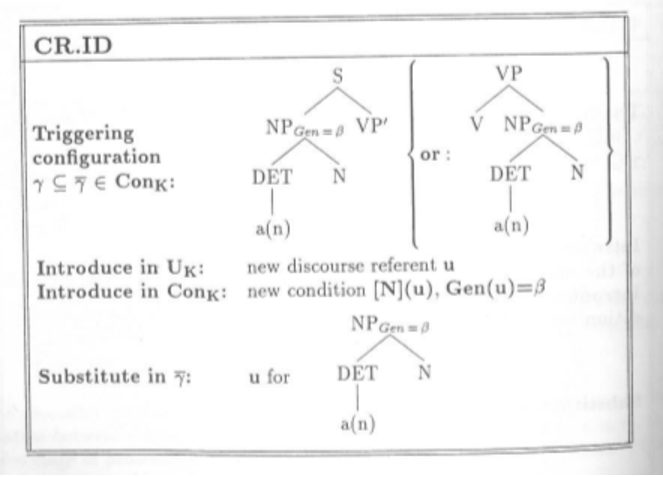
\includegraphics[width=\textwidth]{cr-id}
\end{frame}

\begin{frame}{DRT Construction Rules}
  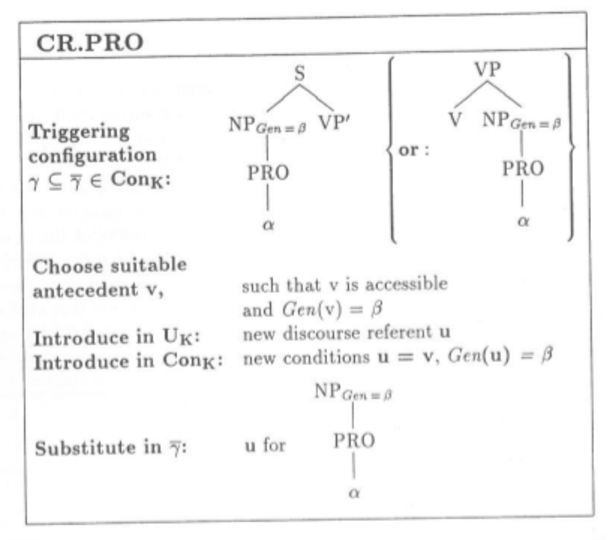
\includegraphics[height=\textheight]{cr-pro}
\end{frame}

\begin{frame}{DRT, Reduction Style}
  $$
  C\left[\ \drs{$x_1$, \ldots, $x_n$}
        {$\gamma_1$ \\
         \ldots \\
         \left( \leaf{$\alpha$} \branch{1}{PRO} \branch{1}{NP$_{Gen=\beta}$}
         \leaf{VP$'$} \branch{2}{S} \tree \right) \\
         \ldots \\
         $\gamma_m$}\ \right]
  \to_{\texttt{CR.PRO}}
  C\left[\ \drs{$x_1$, \ldots, $x_n$, $u$}
        {$\gamma_1$ \\
         \ldots \\
         $u = v$ \\
         $Gen(u) = \beta$ \\
         \left( \leaf{$u$} \leaf{VP$'$} \branch{2}{S} \tree \right) \\
         \ldots \\
         $\gamma_m$}\ \right]
  $$

  where $v$ is a suitable accessible that is accessible and for which
  $Gen(v) = \beta$.
\end{frame}

\begin{frame}[fragile]{DRT, ML Style}
  \begin{lstlisting}
cr_pro (S (NP beta (PRO alpha)) vp') =
  let v = choose (fun v -> gen v = beta) in
  let u = introduce () in
  assert (u = v)
  assert (gen u = beta)
  u
  \end{lstlisting}
\end{frame}

\begin{frame}{DRT, Continuation Passing Style}
  \begin{align*}
    \texttt{CR.PRO}_\beta =
    & \app{\op{choose}}{(\lam{v}{Gen(v) = \beta})}{ \only<2->{&} (\lam{v} \\
    & {\ap{\op{introduce}}{ \only<2->{&} (\lam{u} \\
    & {\app{\op{assert}}{(u = v)}{ \only<2->{&} ( \\
    & {\app{\op{assert}}{(Gen(u) = \beta)}{ \only<2->{&} ( \\
    & {\ap{\eta}{u}})}})}})}})}
  \end{align*}
  \pause
  \pause
  \begin{align*}
    \op{choose} &: (\iota \to o) \to \only<4->{&} (\iota \to \FF(\alpha)) \to \FF(\alpha) \\
    \op{introduce} &: \only<4->{&} (\iota \to \FF(\alpha)) \to \FF(\alpha) \\
    \op{assert} &: o \to \only<4->{&} \FF(\alpha) \to \FF(\alpha) \\
    \eta &: \alpha \to \FF(\alpha)
  \end{align*}
\end{frame}

\begin{frame}{DRT, Philippe de Groote Style}
  \begin{align*}
    \FF(\alpha) &= \gamma \to (\alpha \times \gamma \to o) \to o \\
    \FF(1) &\simeq \gamma \to (\gamma \to o) \to o \quad (= \bar{o}) \\
    \op{choose} &= \lam{f k e \phi}{\appp{k}{(\app{\sel}{f}{e})}{e}{\phi}} \\
    \op{introduce} &= \lam{k e \phi}{\exists x. \appp{k}{x}{e}{\phi}} \quad (= \bar{\exists}\ ) \\
    \op{assert} &= \lam{p k e \phi}{p \land (\appp{k}{e}{\phi})}
  \end{align*}
\end{frame}


\section{Translating to Philippe's work}


\section{Adding new effects --- presuppositions}


\section{Adding new effects --- deixis}


\section{Adding new effects --- expressives}


\end{document}
